\documentclass{beamer}
\usepackage[T1]{fontenc}

\title{PowerEnJoy}
\subtitle{Requirement Analysis and Specifications Document}
\author{Patrizia Porati \\ Tommaso Sardelli}
\date{\today}
\usetheme{CambridgeUS}

\begin{document}
	
	\begin{frame}
		\maketitle
	\end{frame}

%--------------
% INTRODUZIONE 
%--------------
	\begin{frame}
		\frametitle{}
		\begin{block}{Introduction}
			The task we are asked to complete is the definition of a \textbf{software system to manage a car sharing
			service composed by electric cars}. This is going to be a brand new system without any
			legacy software or data to deal with. The idea is that users can register to our platform
			using an internet connected device (computer, smartphone, etc.) and then they are able to
			look for available cars in a certain area. 
			One of the available cars can be reserved and picked up in not more then one hour; at that
			point the user is billed for the time he's using the car.
			Finally, the system can apply discounts or penalties.
		\end{block}
	\end{frame}

%-------------
%USE CASE
%-------------
	\begin{frame} {Use case diagram}
		\includegraphics[height = 0.85\textheight]{figures/UseCaseDiagram-eps-converted-to.pdf}
	\end{frame}

%--------------
%USER INTERFACE
%--------------
	\begin{frame}{User interface}
		\begin{columns}
			\begin{column}{0.4\textwidth}
				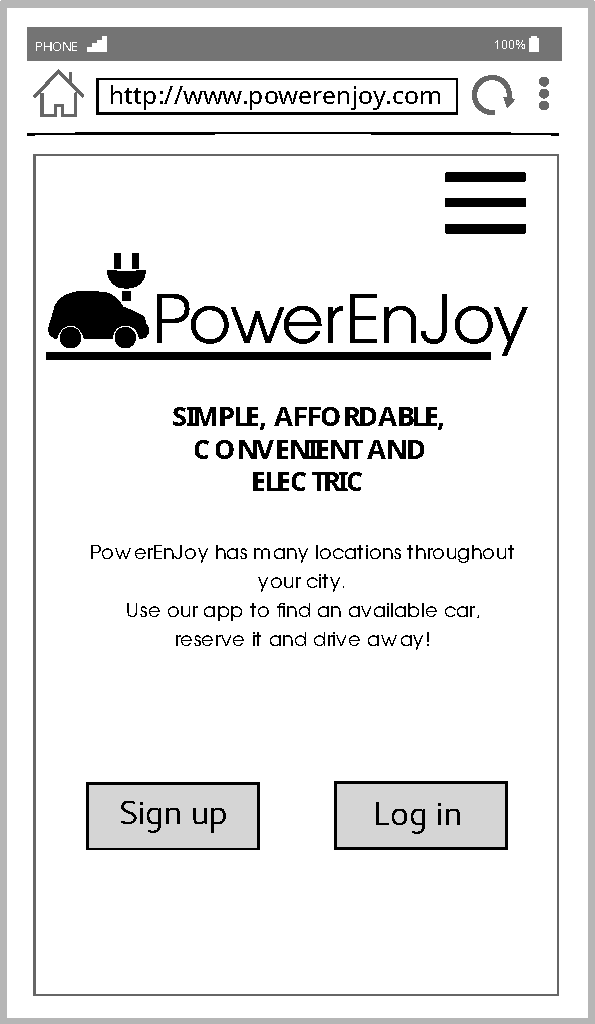
\includegraphics[width=0.9\columnwidth]{figures/homepage.pdf}
			\end{column}
			\begin{column}{0.4\textwidth}
				\textbf{The home page:} \\ both guests and registered user can reach this page. Guest can only sign up, registered user can only log in.
			\end{column}
		\end{columns}
	\end{frame}


	\begin{frame}{\textbf{User interface:} the registration page}
	\begin{columns}
			\begin{column}{0.4\textwidth}
				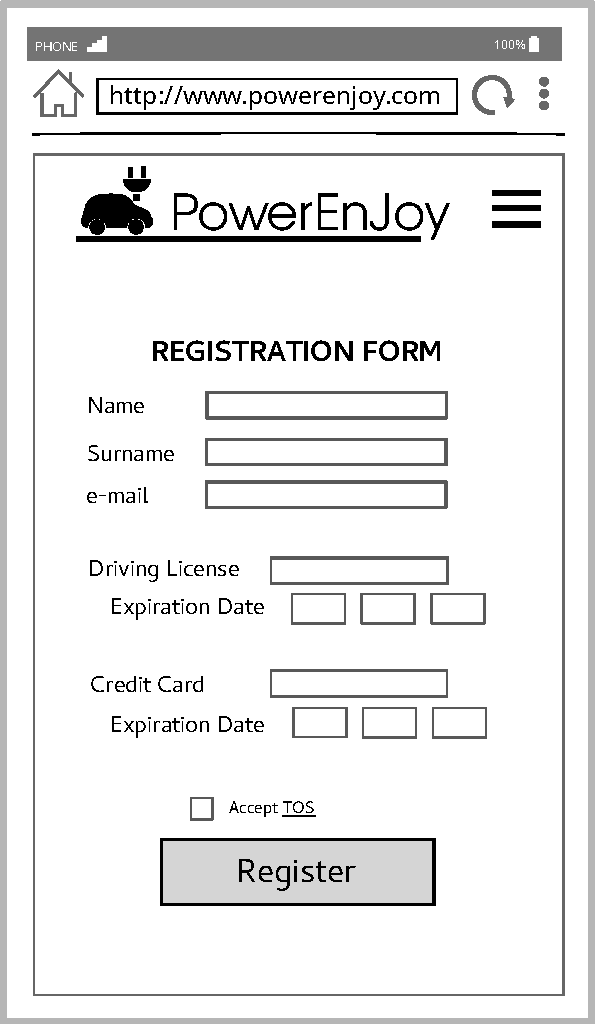
\includegraphics[width=0.9\columnwidth]{figures/sign_up.pdf}
			\end{column}
			\begin{column}{0.5\textwidth}
				\textbf{Goal:} Guests can register to the platform receivin back a login password\\
				\textbf{Requirements:}
				\begin{itemize}
					\item The system shall verify the user's credit card and driving licence are valid
					\item The system shall send a login password to the user who has just signed up in less than 5 minutes. 
				\end{itemize} 
			\end{column}
		\end{columns}
	\end{frame}	

	\begin{frame}{\textbf{User interface:} the login page}
	\begin{columns}
		\begin{column}{0.4\textwidth}
			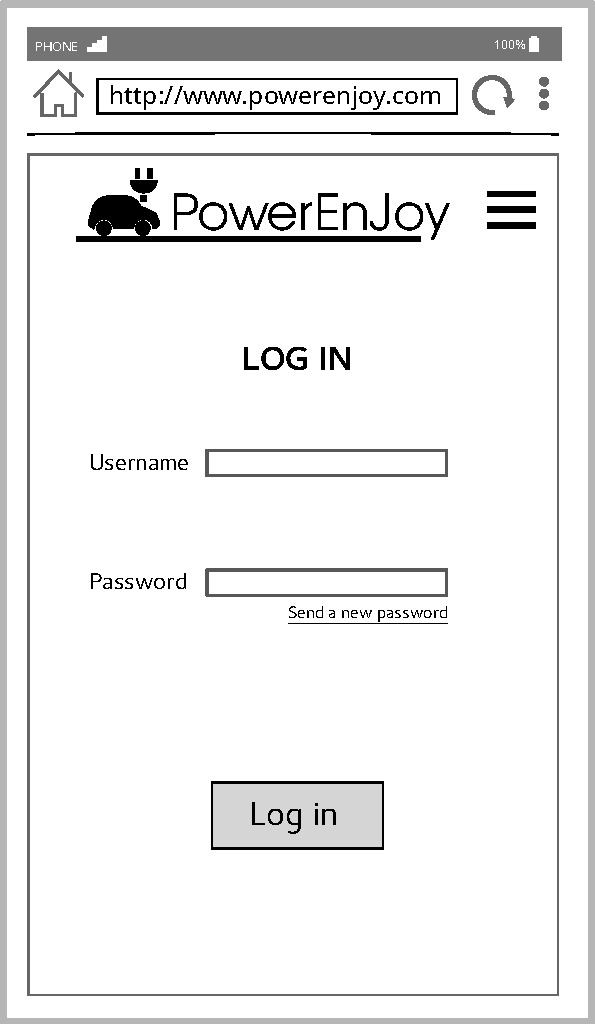
\includegraphics[width=0.9\columnwidth]{figures/login.pdf}
		\end{column}
		\begin{column}{0.5\textwidth}
			Registered user has to log in, in order to use PowerEnJoy services.
		\end{column}
	\end{columns}
	\end{frame}	

	\begin{frame}{\textbf{User interface:} personal profile page}
	\begin{columns}
		\begin{column}{0.4\textwidth}
			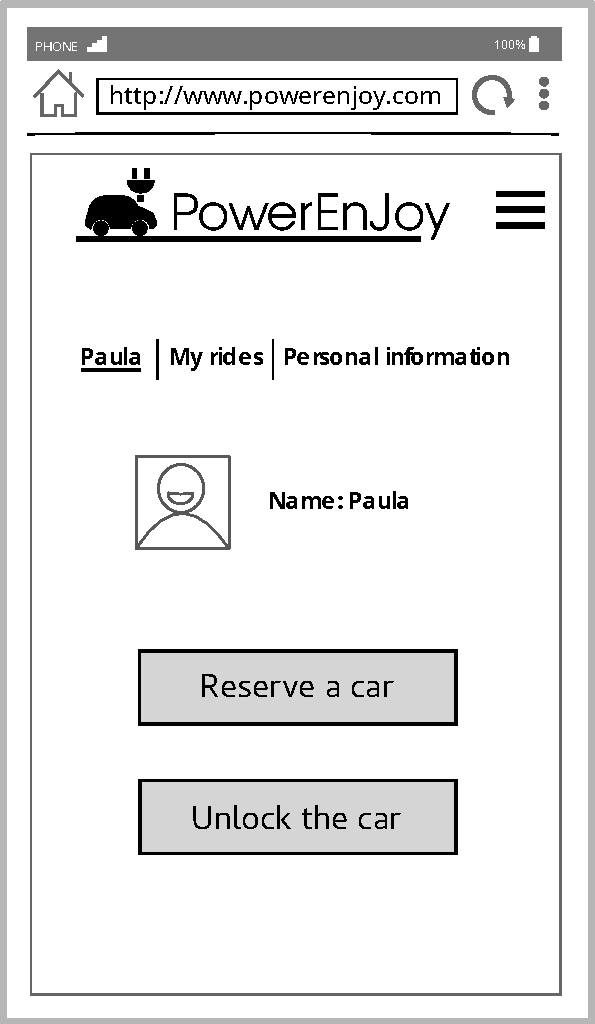
\includegraphics[width=0.9\columnwidth]{figures/profile_page.pdf}
		\end{column}
		\begin{column}{0.5\textwidth}
			\textbf{Goal:} Unlock the car when the user who reserved it is closer than a defined distance\\
			\textbf{Requirements:}
			\begin{itemize}
				\item The system shall not unlock if the distance between the user and the car is greater than the defined distance
			\end{itemize} 
		\end{column}
	\end{columns}
	\end{frame}	

	\begin{frame}{\textbf{User interface:} reservation page}
	\begin{columns}
		\begin{column}{0.4\textwidth}
			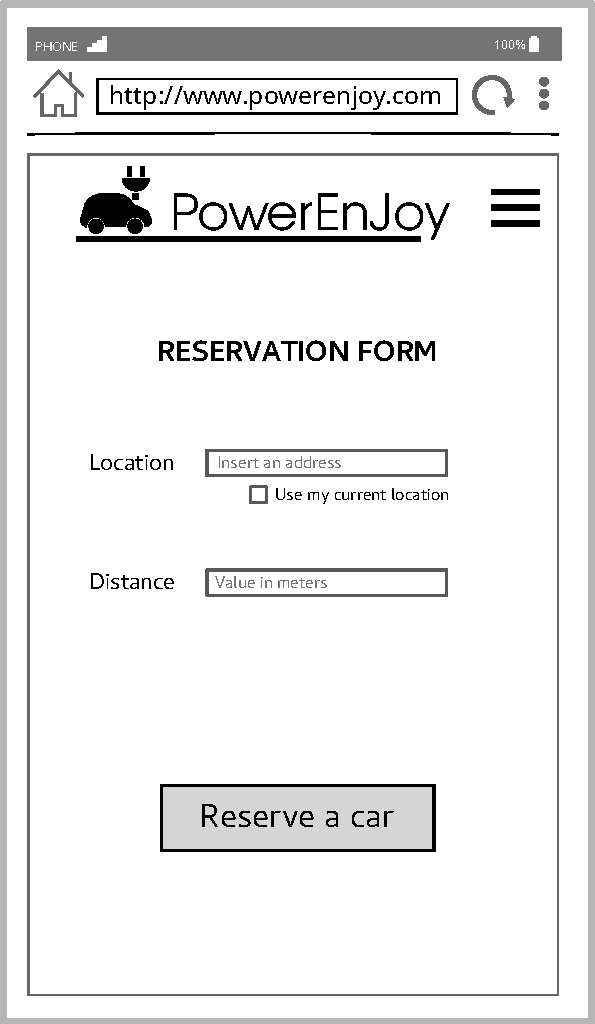
\includegraphics[width=0.9\columnwidth]{figures/reservation.pdf}
		\end{column}
		\begin{column}{0.5\textwidth}
			\textbf{Goal:} Registered users must be able to reserve a single car among all the available cars\\
			\textbf{Requirements:}
			\begin{itemize}
				\item The system shall verify that the user is not receiving more than one car at a time
				\item The system shall verify than the user can select a car only among the list of cars marked as ``available'' in the search radius
				\item The system shall keep track of the time elapsed as soon as the reservation is completed
			\end{itemize} 
		\end{column}
	\end{columns}
	\end{frame}	

	\begin{frame}{\textbf{User interface:} display of the car}
	\begin{columns}
		\begin{column}{0.4\textwidth}
			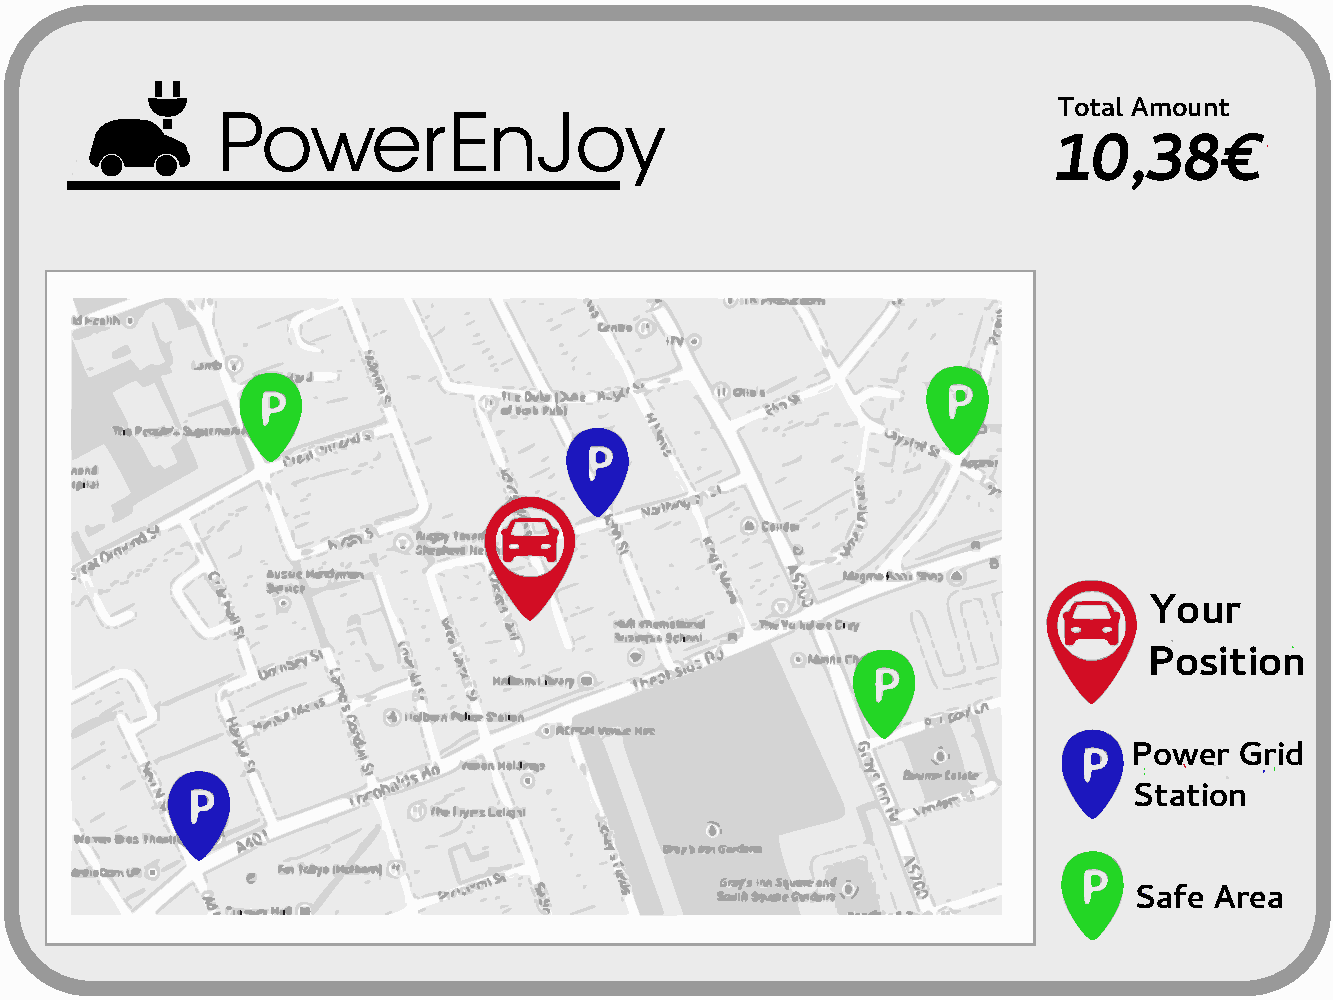
\includegraphics[width=0.9\columnwidth]{figures/screen.pdf}
		\end{column}
		\begin{column}{0.5\textwidth}
			\textbf{Goal:} The car display provides informations about the location of safe areas and power grid stations\\
			\textbf{Requirements:} The system shall send informations to the car about the nearest safe areas and power grid stations based on the current position of the car \\
			\textbf{Glossary:}
			\begin{itemize}
				\item \textit{safe area}: a PowerEnJoy parking slot where the user can leave the car at the end of the ride
				\item \textit{power grid station}: a special safe area with an electric outlet to charge the car battery  
			\end{itemize}
		\end{column}
	\end{columns}
	\end{frame}	

%---------------
% RESERVE THE CAR
%----------------
	\begin{frame}{\textbf{Reserve the car:} use case}
		\begin{block}{Partecipating actors:}
			Registered user: a registered user is a guest that has already signed up.
		\end{block}
		\begin{block}{Entry condition:}
			This use case starts when, after logging in, the registered user clicks on ``\textit{Reserve a car}'' from his/her personal profile page.
		\end{block}
	\end{frame}

	\begin{frame} {\textbf{Reserve the car:} use case}
		\textbf{Flow of events:}\\
			\begin{itemize} 
				\item The registered user clicks on ``\textit{Reserve a car}''
				\item The system shows the reservation form
				\item The user selects where to search the car: choosing if use his/her current location or a specified address (in this case he/she also has to write an address)
				\item The user selects a maximum distance for the car research
				\item The user clicks on ``\textit{Search cars}''
				\item The system searches available cars within the maximum distance indicated from the given location
			\end{itemize}
	\end{frame}

	\begin{frame} {\textbf{Reserve the car:} use case}
		\textbf{Flow of events:}\\
		\begin{itemize} 
			\item The system shows the list of available cars
			\item The user selects one of the cars in the list
			\item The user clicks on ``\textit{Reserve}''
			\item The system changes the status of the car from ``\textit{available}'' to ``\textit{reserved}''
			\item The system displays a confirmation message containing the details of the reservation (time of the reservation, license plate, position, distance from the given location \ldots)
			\item The system displays the user's personal profile page
		\end{itemize}
	\end{frame}
	
	\begin{frame}{\textbf{Reserve the car:} use case}
		\begin{block}{Exit condition:}
			This use case terminates when the confirmation message is shown and the user is redirected on his/her personal profile page.\\
		\end{block}
	\end{frame}

	\begin{frame}{\textbf{Reserve the car:} use case}
		\textbf{Exceptions:}\\
		\begin{itemize}
			\item \textbf{The user doesn't select a location for the car research:} if this exception occurs, the system displays the error message: ``\textit{ERROR: you have to select a location for the car research!}'' and the application goes back to the page where the reservation form is shown.
			\item \textbf{The user writes an inexistent address:} if this exception occurs, the system displays the error message: ``\textit{ERROR: the inserted address doesn't exist!}'' and the application goes back to the page where the reservation form is shown.
			\item \textbf{There aren't cars in the selected area:} if this exception occurs, the system displays the error message: ``\textit{ERROR: there are no cars in the selected area! Please change the maximum distance or the selected location.}'' and the application goes back to the page where the reservation form is shown.
		\end{itemize}
	\end{frame}

	\begin{frame}{\textbf{Reserve the car:} sequence diagram}
		\includegraphics[height=0.9\textheight]{figures/sdRESERVATION-eps-converted-to.pdf}
	\end{frame}

%--------------
% UNLOCK THE RESERVED CAR
%--------------
	\begin{frame}{\textbf{Unlock the reserved car:} use case}
		\begin{block}{Partecipating actors:}
			Registered user: a registered user is a guest that has already signed up.
		\end{block}
		\begin{block}{Entry condition:}
			This use case starts when a registered user who has already reserved a car wants to unlock it, so logs in the application.
		\end{block}
	\end{frame}
	
	\begin{frame} {\textbf{Unlock the reserved car:} use case}
		\textbf{Flow of events:}\\
		\begin{itemize} 
			\item The system displays the user's personal profile page
			\item The user clicks on ``\textit{Unlock the reserved car}''
			\item The system checks the distance between the user and the reserved car
			\item The system change the status of the car from ``\textit{reserved}'' to ``\textit{in use}''
			\item The system unlocks the car
			\item The user gets on the car in less than ten minutes
		\end{itemize}
	\end{frame}
	
	\begin{frame}{\textbf{Unlock the reserved car:} use case}
		\begin{block}{Exit condition:}
			This use case terminates when the system unlocks the car and the user gets in.
		\end{block}
	\end{frame}
	
	\begin{frame}{\textbf{Unlock the reserved car:} use case}
		\textbf{Exceptions:}\\
		\begin{itemize}
			\item \textbf{The user is at more than 3 meters from the car:} if this exception occurs, the system displays the error message: ``\textit{ERROR: you are too far from the car to unlock it! Please go next to the reserved car.}'' and the application shows the user's personal profile page.
			\item \textbf{The user doesn't gets on the car in less than ten minutes:} if this exception occurs, the system locks the car and the ride is considered ended.
		\end{itemize}
	\end{frame}

	\begin{frame}{\textbf{Unlock the reserved car:} sequence diagram}
		\includegraphics[height=0.9\textheight]{figures/sdUNLOCK-eps-converted-to.pdf}
	\end{frame}

%------------------
% THE RIDE
%------------------
	\begin{frame} {\textbf{The ride:} definition}
		\begin{block}{The ride}
		a ride is what follows a reservation when the user picks up the car in time. It begins with the car unlocking, it ends when the car is pared and locked and it keeps track of the user who drove the car and the rime of car usage.
		\end{block}
	\end{frame}

	\begin{frame} {\textbf{The ride:} goals and requirements}
		
			\begin{itemize}
				\item \textbf{Goal:}The user is charged on a per minute basis from the time when the ride begins.\\
				
				\begin{itemize}
					\item \textbf{Requirement:} The system shall keep trak of the time elapsed from the car unlock
					\item \textbf{Requirement:} The system shall update the total cost of the ride on a per minute basis, using the current elapsed time.
				\end{itemize}
				\item \textbf{Goal:} At the end of the ride, the car is locked automatically and the user is charged\\

				\begin{itemize}
					\item \textbf{Requirement:} The system shall lock the car automatically when the car is turned off and there are no more passengers
					\item The system shall wait 5 minutes before charging the user with the final cost in order to consider possible discounts or additional fees
					\item \textbf{Requirement:} The system shall send a notification to the user with information about the ride details and the final cost
				\end{itemize}
			\end{itemize}
	\end{frame}

%-------------
% END THE RIDE
%-------------
	\begin{frame}{\textbf{End the ride} use case}
		\begin{block}{Partecipating actors:}
			Registered user: a registered user is a guest that has already signed up.
		\end{block}
		\begin{block}{Entry condition:}
			This use case starts when the car is parked and the user and all eventual passengers exit the car.
		\end{block}
	\end{frame}
	
	\begin{frame} {\textbf{End the ride:} use case}
		\textbf{Flow of events:}\\
		\begin{itemize} 
			\item The user parks and turns off the car
			\item The user and eventual passengers exit the car
			\item The system locks the car
			\item The system waits five minutes
			\item The system checks the location
			\item The system checks the level of the battery
		\end{itemize}
	\end{frame}

	\begin{frame} {\textbf{End the ride:} use case}
		\textbf{Flow of events:}\\
		\begin{itemize} 
			\item The system checks if the power grid is plugged
			\item The system calculates the total to be paid
			\item The system charges the user the cost of the ride
			\item The system changes the status of the car from ``\textit{in use}'' to ``\textit{available}'' or ``\textit{unavailable}'', based on  car conditions
			\item The system sends the user an e-mail containing all the details of the ride (total cost, discounts, fees, duration, starting location, ending location\ldots)
			\item The user receives the e-mail
		\end{itemize}
	\end{frame}
	
	\begin{frame}{\textbf{End the ride:} use case}
		\begin{block}{Exit condition:}
			This use case terminates when the user receives the e-mail containing the details of his last ride.
		\end{block}
	\end{frame}

	\begin{frame}{\textbf{End the ride:} activity diagram}
		\includegraphics[height = 0.9\textheight]{figures/adENDofRIDE-eps-converted-to.pdf}
	\end{frame}

%--------------
%DISCOUNTS AND PENALITIES
%--------------
	\begin{frame}{\textbf{Discounts and penalities:} activity diagram }
		\includegraphics[height=0.9\textheight]{figures/adDISCOUNTS-eps-converted-to.pdf}
	\end{frame}

	\begin{frame}{\textbf{Discounts and penalities:} goals and requirements}
			\begin{itemize}
				\item \textbf{Goal:} Discourage parking outside of safe areas by charging 80\% more on the ride balance and if that happens, mark the car as unavailable.
				\begin{itemize}
					\item \textbf{Requirement: } The system shall know in advance what are the safe areas and their precise location
				\end{itemize}
				\item \textbf{Goal:} Apply a 10\% discount if there are more than 2 passengers
				\item \textbf{Goal:} Apply a 20\% discount if the car is left with no more than 50\% of battery empty
				\item \textbf{Goal: } Apply a 30\% discount if the car is plugged to the power grid at the end of the ride
				\begin{itemize}
					\item The system shall detect if the car has been plugged to a power grid within 5 minutes from the moment when the car is turned off
				\end{itemize}
				\item \textbf{Goal:} Charge ad additional fee if the car is left more than 3km far from the nearest power grid stations and with less then 20\% of battery left
				\item \textbf{Goal: } Car reservation expires after one hour and a fee is charged to the user.
			\end{itemize}		
	\end{frame}

%---------------
%CLASS DIAGRAM
%---------------
	\begin{frame}{Class diagram}
		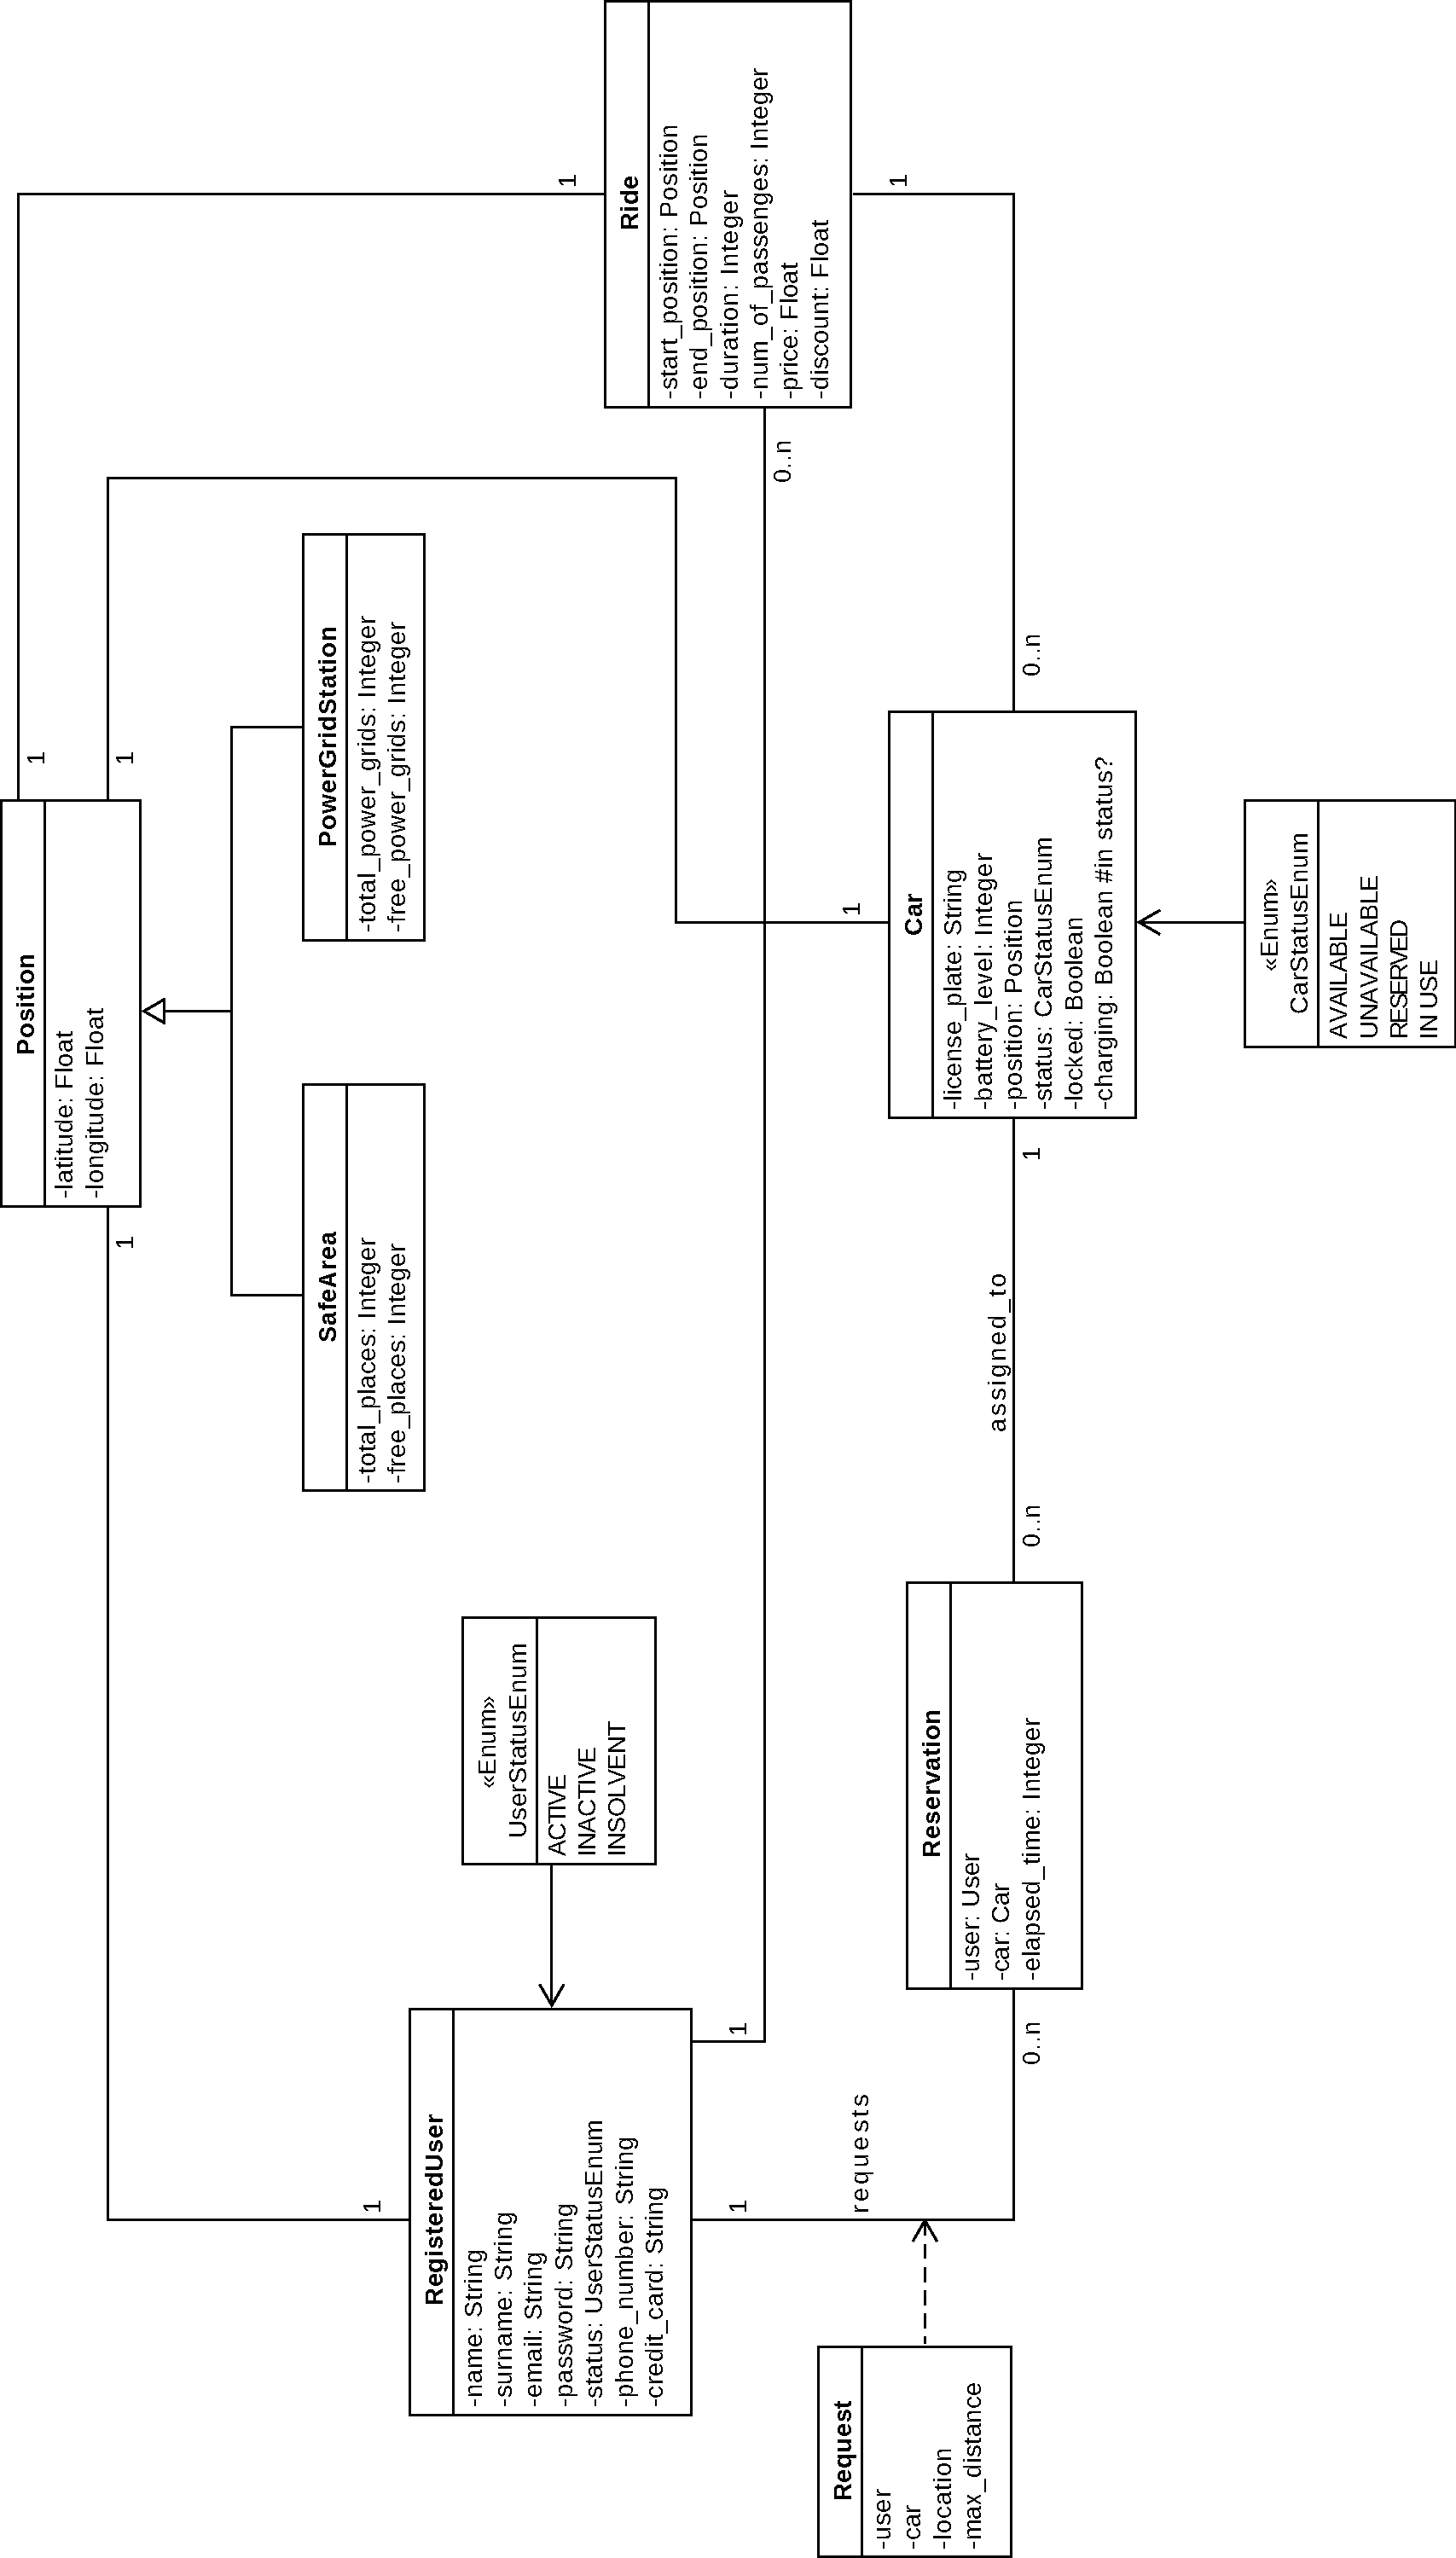
\includegraphics[height=\textwidth, angle=270]{figures/classdiagram.pdf}		
	\end{frame}

\end{document}